\tikzset{every picture/.style={line width=0.75pt}} %set default line width to 0.75pt        

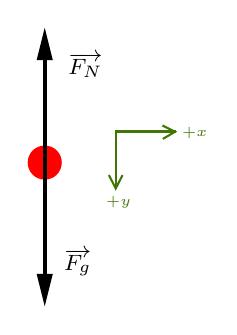
\begin{tikzpicture}[x=0.75pt,y=0.75pt,yscale=-1,xscale=1]
	%uncomment if require: \path (0,300); %set diagram left start at 0, and has height of 300

	%Shape: Ellipse [id:dp9950989906592862] 
	\draw  [color={rgb, 255:red, 255; green, 0; blue, 0 }  ,draw opacity=1 ][fill={rgb, 255:red, 255; green, 0; blue, 0 }  ,fill opacity=1 ] (182.07,109.96) .. controls (182.07,105.7) and (185.53,102.25) .. (189.79,102.25) .. controls (194.05,102.25) and (197.5,105.7) .. (197.5,109.96) .. controls (197.5,114.22) and (194.05,117.68) .. (189.79,117.68) .. controls (185.53,117.68) and (182.07,114.22) .. (182.07,109.96) -- cycle ;
	%Straight Lines [id:da5274227465782517] 
	\draw [line width=1.5]    (189.79,109.96) -- (189.79,49.02) ;
	\draw [shift={(189.79,45.02)}, rotate = 90] [fill={rgb, 255:red, 0; green, 0; blue, 0 }  ][line width=0.08]  [draw opacity=0] (15.6,-3.9) -- (0,0) -- (15.6,3.9) -- cycle    ;
	%Straight Lines [id:da9183971803471973] 
	\draw [line width=1.5]    (189.79,109.96) -- (189.79,175.19) ;
	\draw [shift={(189.79,179.19)}, rotate = 270] [fill={rgb, 255:red, 0; green, 0; blue, 0 }  ][line width=0.08]  [draw opacity=0] (15.6,-3.9) -- (0,0) -- (15.6,3.9) -- cycle    ;
	%Shape: Right Angle [id:dp316002013024695] 
	\draw  [color={rgb, 255:red, 65; green, 117; blue, 5 }  ,draw opacity=1 ] (252.86,94.98) -- (224.03,94.98) -- (224.03,122.5) ;
	\draw  [color={rgb, 255:red, 65; green, 117; blue, 5 }  ,draw opacity=1 ] (227.29,115.98) -- (223.98,122.44) -- (220.7,115.97) ;
	\draw  [color={rgb, 255:red, 65; green, 117; blue, 5 }  ,draw opacity=1 ] (246.5,92.09) -- (252.58,95.12) -- (246.69,98.56) ;


	% Text Node
	\draw (199.67,55.84) node [anchor=north west][inner sep=0.75pt]  [font=\footnotesize] [align=left] {$\displaystyle \overrightarrow{F_{N}}$};
	% Text Node
	\draw (197.63,150.28) node [anchor=north west][inner sep=0.75pt]  [font=\footnotesize] [align=left] {$\displaystyle \overrightarrow{F_{g}}$};
	% Text Node
	\draw (254.44,91.67) node [anchor=north west][inner sep=0.75pt]  [font=\tiny,color={rgb, 255:red, 65; green, 117; blue, 5 }  ,opacity=1 ] [align=left] {$\displaystyle +x$};
	% Text Node
	\draw (217.88,124.61) node [anchor=north west][inner sep=0.75pt]  [font=\tiny,color={rgb, 255:red, 65; green, 117; blue, 5 }  ,opacity=1 ] [align=left] {$\displaystyle +y$};


\end{tikzpicture}